\subsection{Physics motivation for collisions of light ions}
\label{sec:smallAsum}
{ \small
\noindent \textbf{Coordinator}: Z. Citron (Ben-Gurion University of the Negev)

\noindent \textbf{Contributors}:
L. Apolinario (LIP and IST Lisbon),
C. Loizides (Oak Ridge National Laboratory),
G. Milhano (LIP and IST Lisbon, CERN),
A. Milov (Weizmann Institute of Science),
A. Sickles (U. Illinois, Urbana-Champaign)
}

The collision of ion species with A$\ll$A$_\mathrm{Pb}$ is an appealing opportunity to expand the physics programme presented in this document.  The recent \XeXe run of only eight hours has provided valuable input for the physics performance of ion collisions lighter than Pb at the LHC.  Broadly, the advantages of using A$\ll$A$_\mathrm{Pb}$  collisions are twofold: smaller collision systems sample key physical parameters beyond what can be probed with \PbPb and \pPb collisions, and they allow higher luminosity running to maximize the accumulation of rare events in heavy-ion collisions.  This higher luminosity could enable a high-precision paradigm for currently rare observables in \PbPb collisions as well as the study of observables totally inaccessible in \PbPb collisions.        
A two-pronged scenario is envisioned composed of a short run of \OO  ($A=16$) and longer running of a species of intermediate A.  The choice of the intermediate species will be dictated by the competition of increased luminosity with lower A against the goal of studying the properties of an extended QGP system. Optimizing the choice of species will require further study from the accelerator, experimental, and theoretical communities; in this document \ArAr ($A=40$) collisions are considered as a test-case for the choice of intermediate ion.

Section \ref{sec:lightions} describes the technical capabilities of the LHC to provide lighter-ion collisions, as well as describing the expected performance for several different ion species.
For example, for \ArAr the expectation for one month of collisions is 1080 $\invnb$ ($p$=1.5).  In order to compare across different collisions species we consider the \textit{nucleon--nucleon} integrated luminosity per month of running, which could be larger by a factor 3--23 (for $p$=1.2--1.9) with respect to \PbPb collisions, \textit{i.e.} one month of \ArAr collisions would be equivalent to 25--80 $\invnb$ of \PbPb collisions. This gain would be the same in all centrality classes (defined in terms of percentiles of the hadronic cross section).
Section \ref{sec:flow_sizedep} discusses flow measurements possible using smaller species.  A discussion of the role light ion collisions can play for low-$x$ and nPDF studies is found in Sect.~\ref{sec:nPDF_lightions}.  The implications of \ArAr collisions for the study of light-by-light scattering are discussed in Sect.~\ref{sec:upc}.  The choice of the ion species for the HE-LHC is discussed in Sect.~\ref{sec:HELHC}.

Even a short \OO run can help clarify the uncertainty concerning the onset of QGP or QGP-like phenomena in high-multiplicity pA and pp collisions discussed in section \ref{sect:smallsystems_OO}.  The search for basic properties associated with the QGP in \OO collisions should complement the searches in \pp and \pPb collisions.% systems, \textit{i.e.} if they can not be observed in \OO there should be no reasonable expectation of observing them in smaller collisions systems.  
In particular, the \OO system has well-understood collision geometry as described in detail in Sect.~\ref{sect:smallsystems_OO}, enabling the study of collisions with low values of $\langle N_{\rm part}\rangle$ that are difficult to select and study in \PbPb collisions and that are similar to those estimated for high-multiplicity \pPb events. Colliding \OO at the LHC naturally dovetails with \pO collisions whose significance for the cosmic-ray community is detailed in section \ref{sec:pOcosmic}.

Complementing \PbPb collisions, 
the possibility of high-luminosity extended LHC runs with intermediate-A nuclei (e.g.\ArAr)
is a promising long-term option.
%In addition to being a new system and thereby providing another data-point for observables that probe different geometries (see \textit{e.g.} Sect.~\ref{sec:flow_sizedep}),
The chief promise of \ArAr collisions is the possibility of reaching much higher luminosity than \PbPb collisions while still producing a QGP over an extended volume of $\sim 1000$~fm$^3$ in central events. Based on an MC Glauber simulation \cite{Loizides:2017ack}, the mean number of participants expected, $\langle N_{\rm part}\rangle$, for \ArAr ranges from  $\sim 7$ for 60--80\% centrality to $\sim 70$ for 0--5\% centrality collisions.  
QGP effects are observed in \PbPb collisions with similar number of participants \cite{Sirunyan:2018eqi, ATLAS-CONF-2018-007}.  In addition, the much lower underlying event multiplicity in \ArAr relative to central \PbPb collisions is expected to lead to reduced  systematic uncertainties for several observables, from reconstructed jets to all signal affected by large combinatorial backgrounds.  These features, combined with the possibility to increase the nucleon--nucleon luminosity by more than one order of magnitude, make \ArAr collisions an extremely attractive option for hard probe measurements that in \PbPb collisions are `statistics starved' or impossible, such as top quarks for QGP studies as outlined in \cite{Apolinario:2017sob}.  Figure \ref{fig:boosted_tops} extends the analysis to lighter nuclei and shows that one month of \ArAr collisions, with nucleon--nucleon luminosity equivalent to 25--80~$\invnb$ for \PbPb, allows a similar physics reach as the entire \PbPb future programme ($13~\invnb$), namely to probe the QGP density evolution up to a time of about 1.5--2~fm/$c$.  Top quark studies in \ArAr collisions in the context of constraints on nPDFs are detailed in section \ref{sec:nPDF_top}.
\begin{figure}
\centering
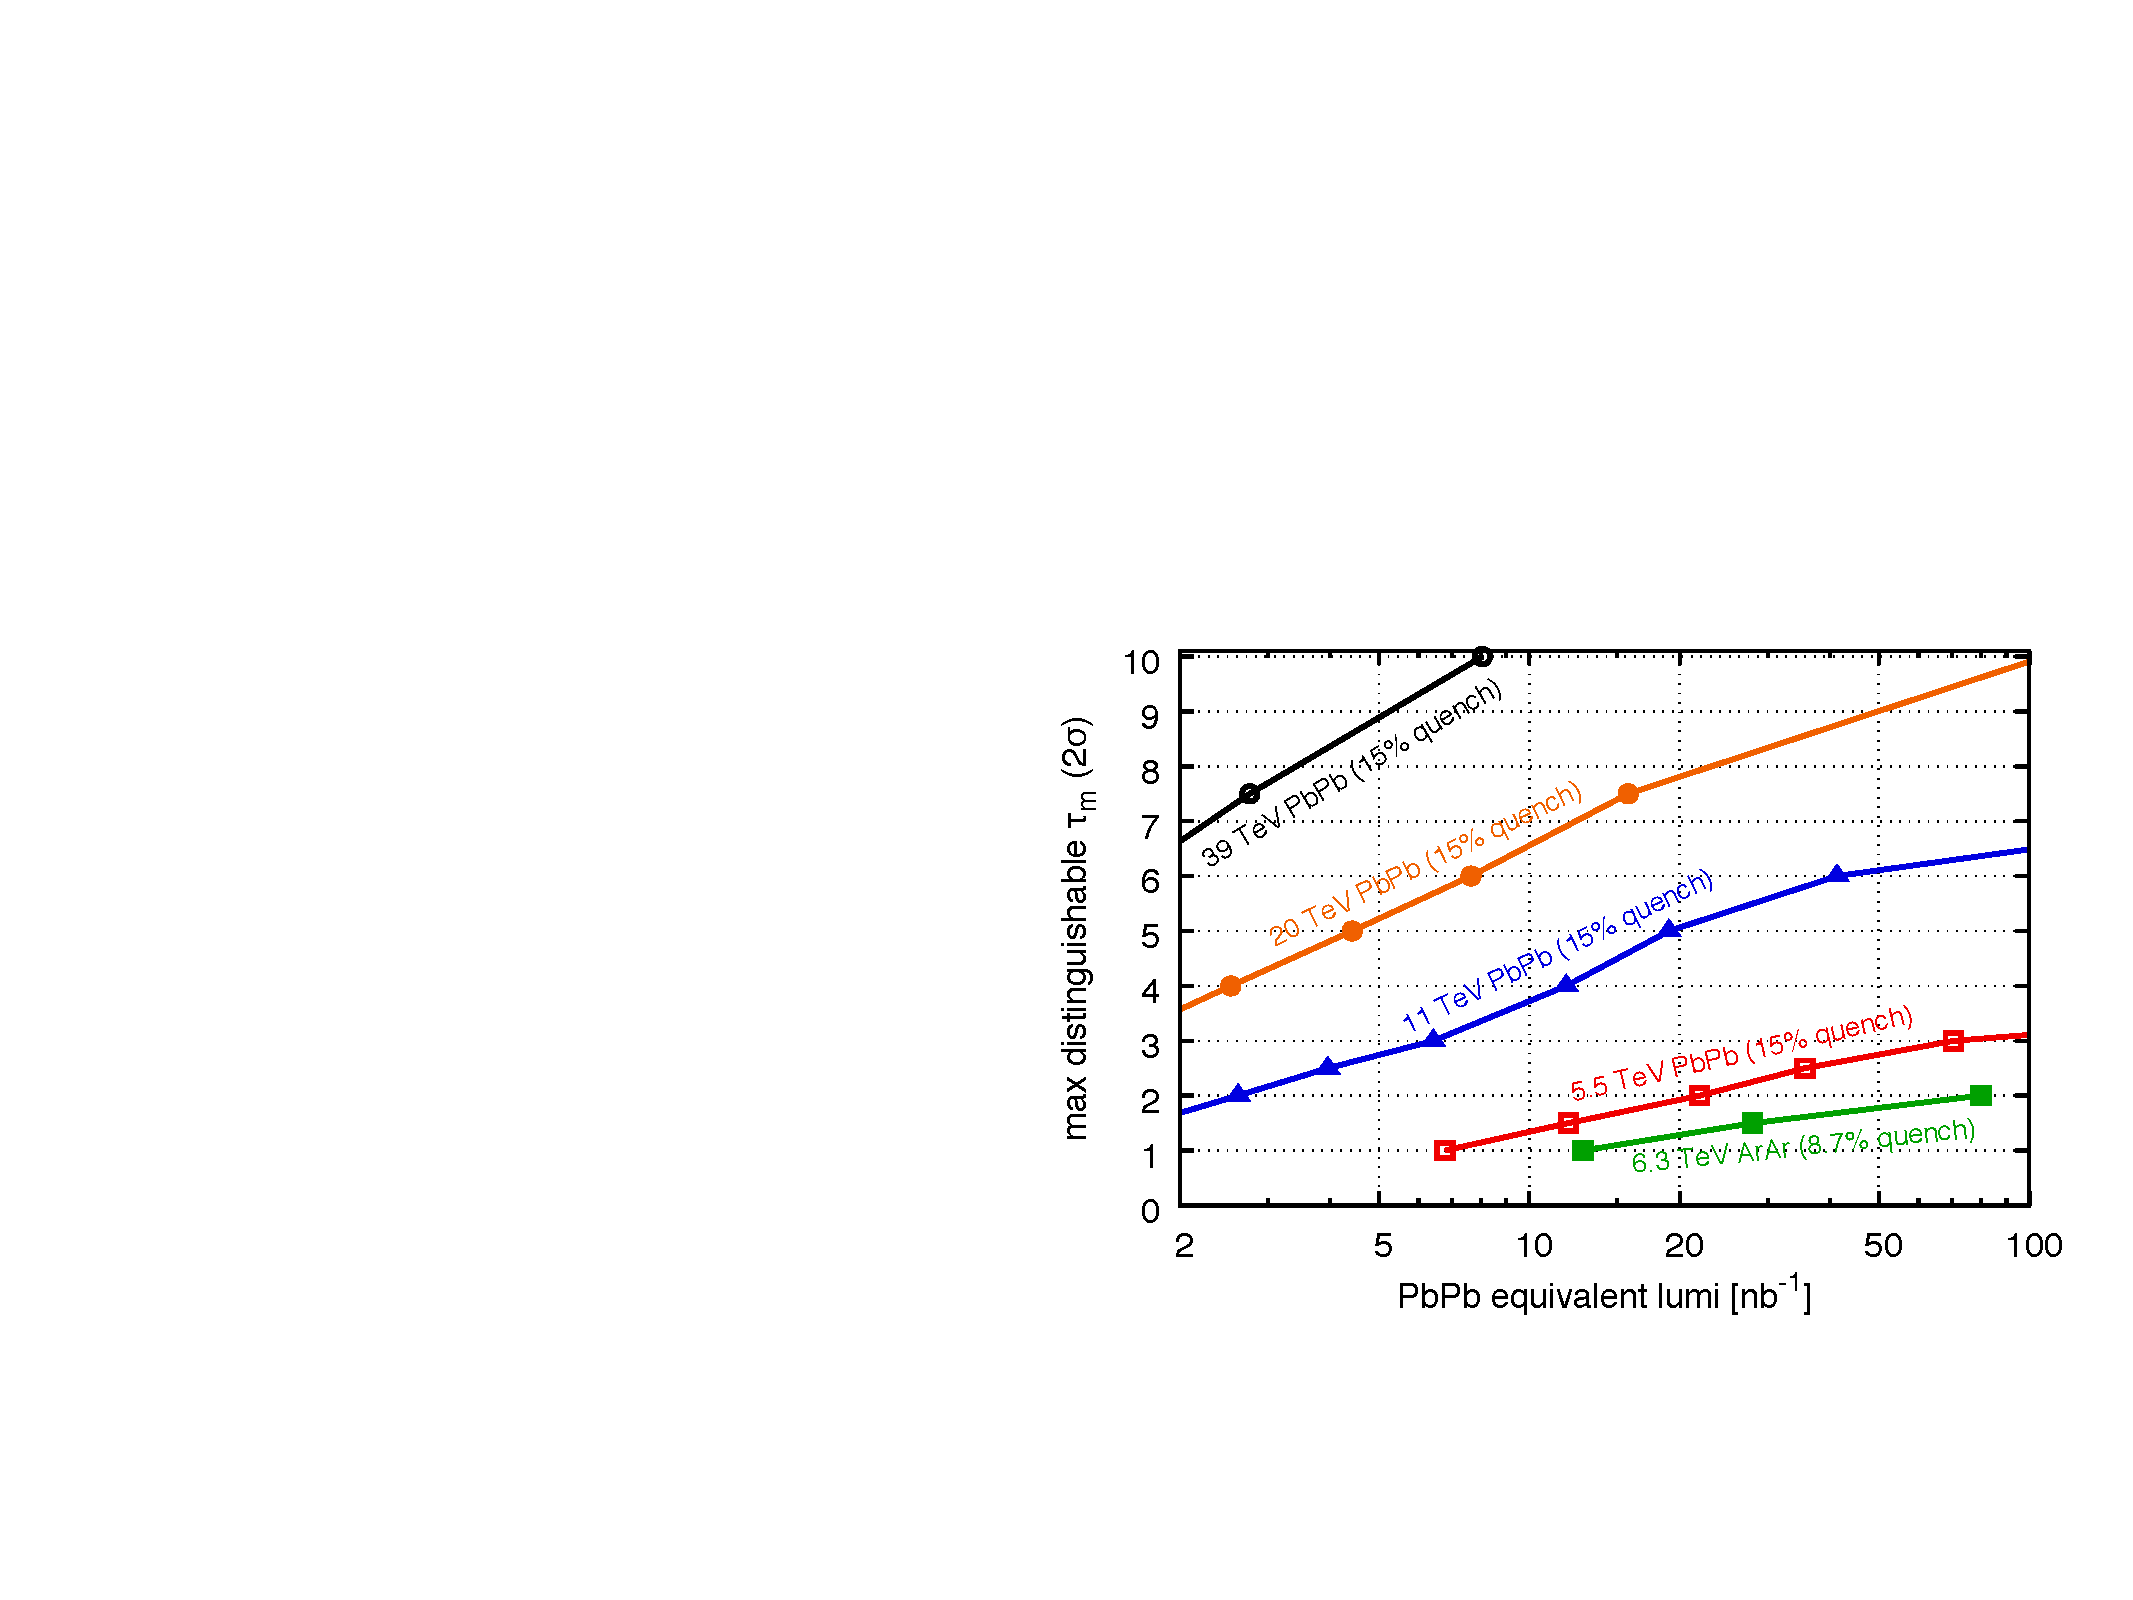
\includegraphics[width=0.68\linewidth]{\main/smallAexec/fig/top_plot}
\caption{Maximum medium lifetime that can be distinguished from a full quenching baseline with two standard deviations (2 $\sigma$), as a function of luminosity for different species and collider energies. The luminosity on the $x$-axis is maintaining an equal number of nucleon-nucleon collisions. A single \ArAr run is expected to provide $\sim$ 25--75 $\invnb$ of \PbPb equivalent luminosity.}
\label{fig:boosted_tops}
\end{figure}

Studies with $Z$ bosons are representative examples of the types of measurements that may be undertaken in a lighter ion rare-probes programme.  In Figure \ref{fig:Zreach} the expected number of $Z$ boson candidates (assuming a selection similar to that used by ATLAS and CMS in previous studies) for one month of heavy ion running  as a function of $\langle N_{\rm part}\rangle$ is shown for several different lighter ion species, and compared with the expectation for the full \PbPb and \pPb programmes.  The figure demonstrates that the overall yield of $Z$ bosons would be considerably higher for one \ArAr run than for several years of \PbPb running including both a sufficient number of candidates to study low $\langle N_{\rm part}\rangle$ collisions unreachable with \PbPb collisions as well as moderate $\langle\Npart\rangle$ values in which QGP formation is expected.  $Z$ bosons are a powerful tool to probe the properties of the QGP in particular in $Z$+jet events.  
\begin{figure}
\centering
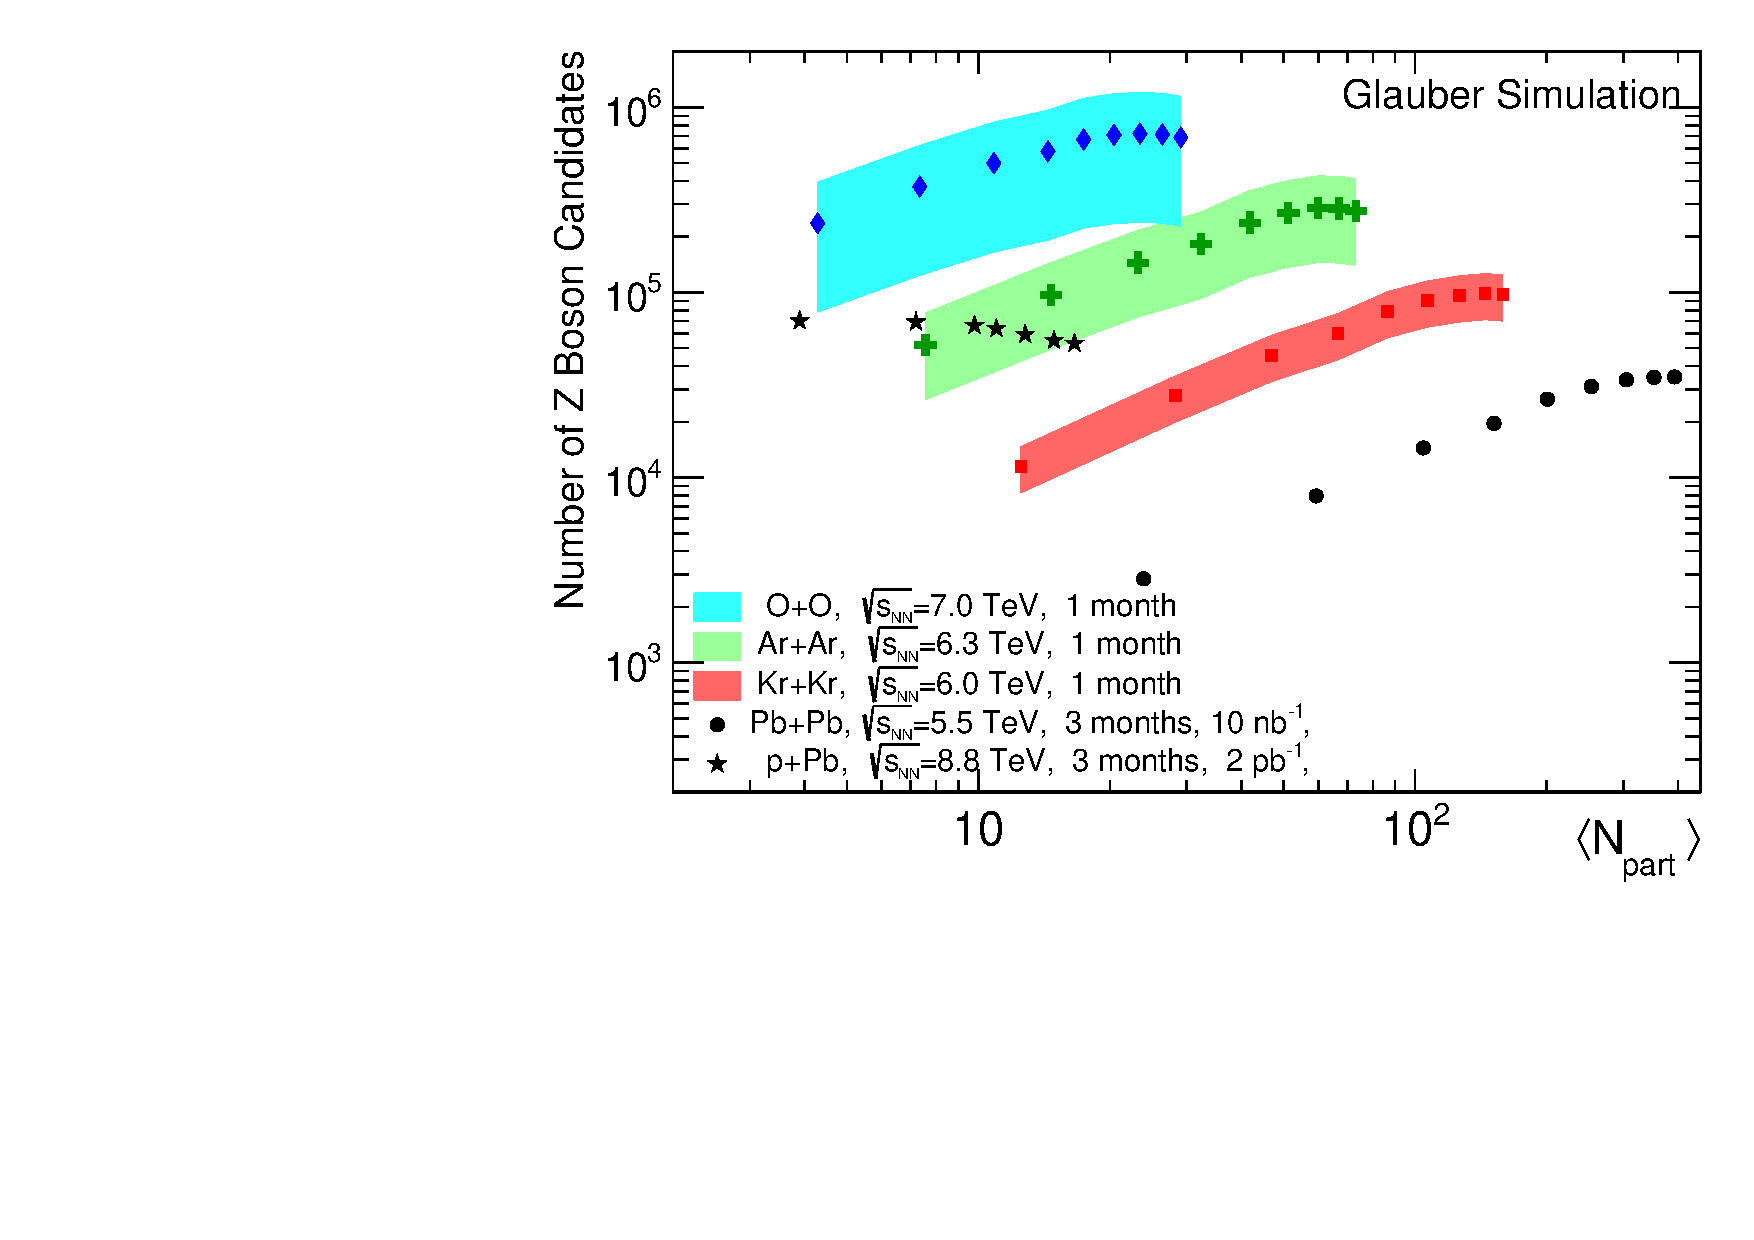
\includegraphics[width=0.68\linewidth]{\main/smallAexec/fig/Zcentreach}
\caption{
The number of $Z$ bosons as a function of $\langle N_{\rm part}\rangle$ expected for one full heavy-ion run at the LHC for several collisions species.  The $Z$ bosons are reconstructed via the di-lepton decay channel with leptonic $\pT>20$~GeV$/c$ and $|\eta|<2.5$, and a mass selection of $66<M_{\ell\ell}<116$~GeV.  Luminosities shown for \PbPb and \pPb correspond to several years of running.  The central values correspond to $p=1.5$ as discussed in section \ref{sec:lightions}, with the uncertainties representing a variation of $p$ down to 1 and up to 1.9.
\label{fig:Zreach}}
\end{figure}

$Z$+jet events were simulated in the 10\% most central events in \ArAr collisions using JEWEL \cite{Zapp:2009ud} to estimate the expected jet-quenching effects.  Figure \ref{fig:ArAr_xjz} shows the distribution of $x_{jZ}$, the ratio of the jet transverse momentum to that of the $Z$ boson for 0--10\% centrality \ArAr events, as well as \pp collisions and 0--10\% centrality \PbPb events ($N_{\rm part} = 356$, $T=360$ MeV at thermalization time $\tau = 0.55$ fm/$c$ for $\sqrt{s}=5.5$ TeV).  The $Z$ boson must have \pt $>$ 60 GeV/$c$ and be back-to-back ($\Delta\varphi > 7/8\pi$) to a jet with \pt $>$ 30 GeV/$c$.  The Figure clearly shows that for this observable the jet-quenching phenomena observed in \PbPb collisions as modelled by JEWEL are present also in \ArAr collisions.  This demonstrates the potential of the \ArAr (or a similar) collision system for a heavy ion rare probes programme.% with a much larger dataset than the LHC \PbPb program.
\begin{figure}
\centering
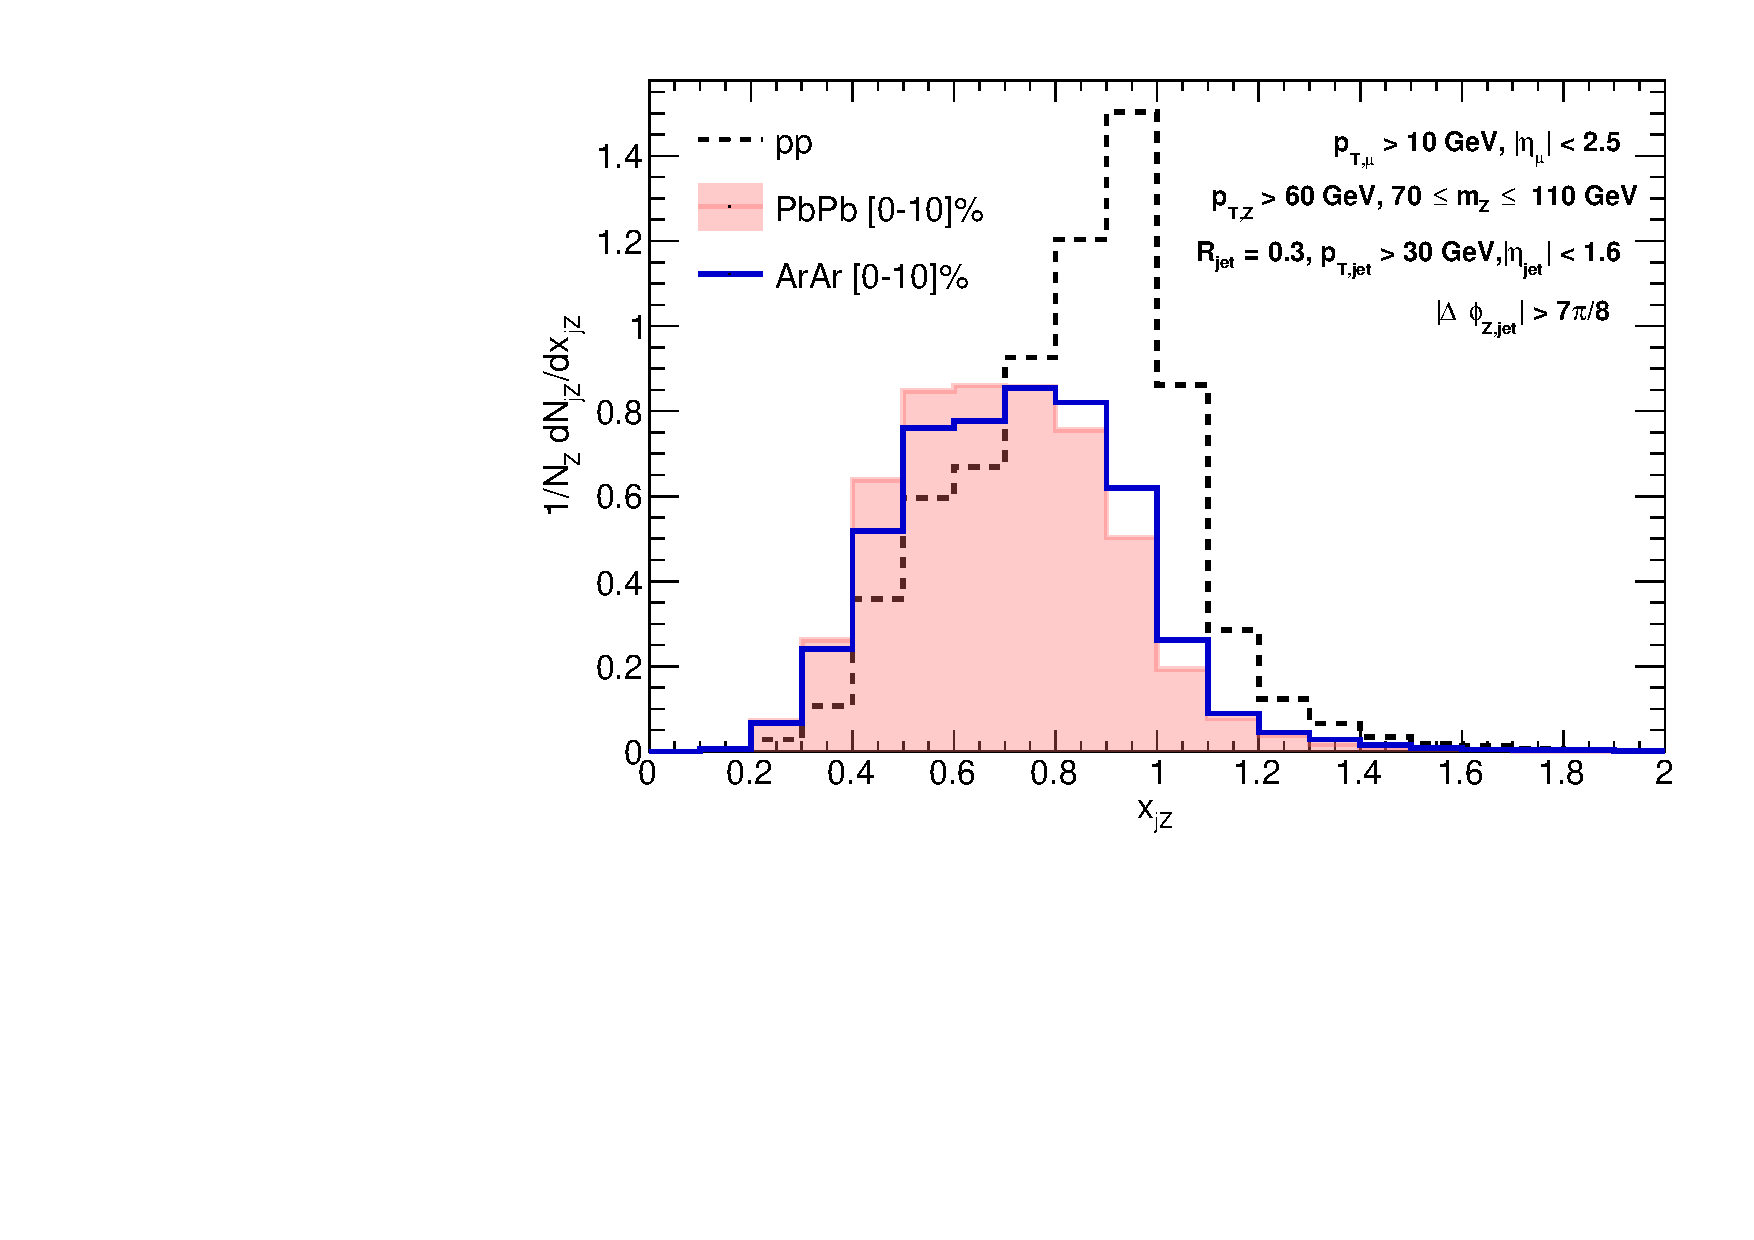
\includegraphics[width=0.48\linewidth]{\main/smallAexec/fig/Zjetassym}
\caption{
The $x_{jZ}$ distribution for pp, \PbPb, and \ArAr collisions calculated with JEWEL.  The 10\% most central events are shown for \PbPb and \ArAr.  \ArAr collisions are calculated as $N_{\rm part} = 60$, $T=318$ MeV at thermalization time $\tau = 0.63$ fm/$c$ for $\sqrt{s}=6.3$ TeV.  The $Z$ boson must have $\pt > 60$~GeV/$c$ and be back-to-back ($\Delta\varphi > 7/8\pi$) to a jet with $\pt > 30$~GeV/$c$.    
\label{fig:ArAr_xjz}}
\end{figure}